% =========================================================================
%  Biological Penalty Sharpness Bounds the Value of In-Season Replanning
%  in Multi-Field Hybrid Maize Seed Production
%
%  NOTE ON FORMAT: this file reproduces IEEEtran conference style using the
%  standard article class, so it compiles without IEEEtran.cls installed.
%  Conventions follow the supplied reference paper: full-width roman title,
%  a grid of author blocks, bold abstract and index terms with run-in italic
%  labels, centred small-caps section headings, "TABLE N" plus a small-caps
%  caption set ABOVE each table, and "Fig. N." captions set BELOW figures.
%  To submit, drop the body into the conference's official IEEEtran template.
% =========================================================================
\documentclass[10pt,twocolumn]{article}

\usepackage[letterpaper,top=0.75in,bottom=1.0in,left=0.625in,right=0.625in,
            columnsep=0.25in]{geometry}
\usepackage{times}
\usepackage{amsmath,amssymb}
\usepackage{graphicx}
\usepackage{booktabs}
\usepackage{algorithm}
\usepackage{algorithmic}
\usepackage[hidelinks]{hyperref}
\usepackage[labelsep=period]{caption}
\usepackage{titlesec}
\usepackage{balance}

\setlength{\parindent}{1em}
\setlength{\abovedisplayskip}{4pt}
\setlength{\belowdisplayskip}{4pt}

% ---- section headings: centred, small caps, Roman numerals -------------
\renewcommand{\thesection}{\Roman{section}}
\renewcommand{\thesubsection}{\Alph{subsection}}
\renewcommand{\thesubsubsection}{\arabic{subsubsection}}

\titleformat{\section}[block]
  {\normalfont\normalsize\centering\scshape}{\thesection.\quad}{0em}{}
\titlespacing*{\section}{0pt}{10pt plus 2pt minus 2pt}{6pt}

\titleformat{\subsection}[block]
  {\normalfont\normalsize\itshape}{\thesubsection.}{0.6em}{}
\titlespacing*{\subsection}{0pt}{8pt plus 1pt minus 1pt}{4pt}

\titleformat{\subsubsection}[runin]
  {\normalfont\normalsize\itshape}{\thesubsubsection)}{0.5em}{}[:]
\titlespacing*{\subsubsection}{\parindent}{4pt}{0.5em}

% ---- captions: tables above in small caps, figures below ---------------
\captionsetup[table]{position=top,labelsep=newline,justification=centering,
                     font=sc,labelfont=sc,skip=3pt,textformat=simple}
\captionsetup[figure]{position=bottom,font=small,labelfont=normalfont,
                      labelsep=period,skip=5pt,justification=justified}
\renewcommand{\tablename}{Table}
\renewcommand{\thetable}{\Roman{table}}
\renewcommand{\figurename}{Fig}

% ---- IEEE-style run-in abstract (no centred heading, no extra margins) --
\renewenvironment{abstract}
  {\small\bfseries\noindent\textit{Abstract}---\ignorespaces}
  {\par}

\newcommand{\TSI}{\mathrm{TSI}}
\newcommand{\EVPI}{\mathrm{EVPI}}
\newcommand{\VSS}{\mathrm{VSS}}

% ---- title block -------------------------------------------------------
\title{\vspace{-2.2em}\normalfont\LARGE
Optimised Sowing Scheduling for Multi-Field\\
Hybrid Maize Seed Production under\\
Anthesis-Synchrony Constraints}

% Four authors, set as a 2x2 grid. The department name is long, so a single
% row of four would crush each column; the grid keeps the lines unbroken.
\newcommand{\authblock}[2]{%
  \begin{minipage}[t]{0.43\textwidth}\centering
  \normalsize #1\\[2pt]
  \small Dept. of CSE in IoT, Cybersecurity including Blockchain\\
  \small Dayananda Sagar Academy of Technology and Management\\
  \small Bengaluru, India\\
  \small #2
  \end{minipage}}

\author{%
  \begin{tabular}{@{}c@{\hspace{3em}}c@{}}
  \authblock{C. Tejas}{tejasshekar29@outlook.com} &
  \authblock{Mayur Adiga}{adigamayur@gmail.com} \\[14pt]
  \authblock{Pavan Kumar Nayak}{nayakpavan0099@gmail.com} &
  \authblock{Kishore Kumar N.~H.}{kishoreekumarrnh05@gmail.com}
  \end{tabular}}

\date{}

\begin{document}
\twocolumn[
  \begin{@twocolumnfalse}
  \maketitle
  \vspace{-1.0em}
  \end{@twocolumnfalse}
]

\begin{abstract}
\small\bfseries
Hybrid maize seed is produced on many isolated contract fields, but the
sowing of the two parent lines is carried out by one supervised crew, because
the row pattern and the staggered parent dates are what make the product.
The day a field is sown fixes its thermal-time trajectory, hence the
flowering dates of both parents, hence whether their pollen and silk windows
overlap at all --- field data report seed yield falling 29--57\% as the
tasseling--silking interval widens. Sequencing and biology are therefore
inseparable, and rain closes fields unpredictably during the window. We
formulate this as a two-stage stochastic scheduling problem, score it with a
published measured yield response, take flowering dates from CERES-Maize, and
evaluate on twenty-one observed seasons at a working Indian seed-production
site with leave-one-season-out evaluation. ABSTRACT\_FINDING We also ask
whether the reported marginality of in-season replanning in agriculture is
general or an artefact of the response surface it was measured on, and give a
screening rule, computable before any software is written, for when to add
replanning to the optimiser. Model biology is validated against CIMMYT's
published sowing intervals for six tropical hybrids, reproduced to within
1.5~days from data that played no part in building it. Code, weather and
results are released.
\end{abstract}

\vspace{2pt}
\noindent{\small\textit{\textbf{Index Terms}}\textbf{---precision agriculture,
hybrid seed production, anthesis synchrony, flowering synchrony, stochastic
scheduling, rolling-horizon optimisation, value of information.}}
\vspace{6pt}

% =========================================================================
\section{Introduction}
% =========================================================================

Decision-support tools in agriculture increasingly promise to adapt: to
ingest sensor and weather data during the season and revise the plan as
conditions change. The premise is intuitive. The evidence is mixed.

Kelly \textit{et al.}~\cite{kelly2023} re-optimised irrigation strategies at
several points within each season using AquaCrop-OSPy and found that fixed
heuristics already captured more than 90\% of the profit available under
perfect seasonal foresight; in-season adaptation added less than five percent,
and they recommended prioritising fixed strategies because they are simpler to
design, communicate and implement. Becker \textit{et al.}~\cite{becker2026}
compared a genetic algorithm optimising a fixed seasonal strategy against
model predictive control adapting daily, across 21 stochastic weather
scenarios spanning normal conditions to extreme drought, and reported that the
fixed strategies outperformed adaptive control in all 21.

These are careful studies and we do not dispute them; we question their
scope. Both examine water, and water stress accumulates gradually: a plant
irrigated two days late is stressed, not lost. Under such a response a fixed
plan with a safety margin absorbs most of the weather risk before the season
begins, leaving little for adaptation to recover.

Not every operation behaves this way. Hybrid seed production depends on a
coincidence: the male parent must shed pollen while the female is receptive.
Maize pollen stays viable 18--24 hours and the stigma is receptive for two to
three days~\cite{marahatta2025}. If the windows miss, no seed forms, and the
loss is close to total rather than proportional to the delay --- field
experiments report seed yield falling 29--57\% as the tasseling--silking
interval (TSI) widens~\cite{marahatta2025}.

This paper asks a single question:

\begin{quote}
\itshape Does the limited value of in-season replanning reported for
irrigation persist when the biological outcome responds sharply, rather than
gradually, to timing error?
\end{quote}

Answering it requires a scheduling problem in which timing error is both
costly and hard to avoid, and we use one that has not previously been
formulated. A hybrid seed company runs many isolated contract fields but very
few supervised sowing units, because the male-to-female row pattern and the
staggered sowing of the parent lines are what make the product and are not
left to growers. One unit starts only a few fields per day, and the day a
field is started sets the thermal-time trajectory of both parents, hence
their flowering dates, hence whether that field produces seed. Sequencing and
biology are inseparable, and rain closes fields unpredictably during the
window.

\subsection{Contributions}

\begin{enumerate}
\itemsep1pt
\item We show that optimising which field a shared sowing crew serves on
which day produces materially more hybrid seed than current practice, which
uses correct per-hybrid offsets but sequences fields naively. The mechanism
is crew throughput: naive sequencing saturates at a fixed number of fields
however many are offered, while the optimised plan keeps placing them.
\item We formulate multi-field hybrid maize seed sowing as a two-stage
stochastic scheduling problem coupling a shared sowing resource to
parent-specific flowering synchrony, under an explicit non-anticipativity
constraint. The cost of a schedule is not lateness against a fixed ideal date
but the induced mismatch between two weather-dependent flowering events.
\item We score schedules with a published, measured yield response rather
than an assumed objective, take flowering dates from CERES-Maize, and
evaluate on twenty-one observed seasons at a real seed-production site with
leave-one-season-out evaluation.
\item We quantify the additional value of in-season replanning against a
\emph{robust} static optimum rather than a naive baseline, and show it is
conditional on two measurable quantities: the curvature of the biological
penalty, and resource pressure --- the latter non-monotonically. This yields
a screening rule a producer can evaluate with arithmetic.
\item We introduce a one-parameter sharpness family that holds the yield
optimum fixed while varying penalty curvature, and use it to map the
boundary of the Kelly--Becker conclusion, reproducing their null at its flat
end on our own farms.
\item We give a conditioning scheme --- rolling-horizon replanning on
historical analogues --- that preserves non-anticipativity when the objective
comes from a year-indexed crop model.
\item We validate the model's biology against an independent CIMMYT dataset,
and release the simulator, weather, scripts and results.
\end{enumerate}

% =========================================================================
\section{Related Work}
% =========================================================================

\subsection{Flowering synchrony and how practitioners manage it}

The agronomic literature on anthesis synchrony --- \emph{nicking}, in the
seed trade's own terminology --- is mature, practical, and almost entirely
single-field. Marahatta \textit{et al.}~\cite{marahatta2025} staggered male
inbred sowing across two seasons and two hybrids and fitted seed yield
against TSI directly; their regressions are the empirical foundation of our
objective. Chassaigne-Ricciulli \textit{et al.} quantified effective seed
yield against parental synchrony for CIMMYT three-way-cross
hybrids~\cite{chassaigne2021} and developed sowing recommendations for
single-cross hybrids~\cite{chassaigne2020}. Fonseca \textit{et
al.}~\cite{fonseca2004} and Schneider~\cite{schneider2005} modelled kernel
set from pollen--silk overlap, and Laurent \textit{et al.}~\cite{laurent2025}
integrate a crop growth model with whole-genome prediction to forecast
synchrony and recommend a differential planting interval.

Two features of this literature bear directly on our formulation. First,
practitioners manage nicking with \emph{two} levers, not one: staggered
sowing, and supplementary nitrogen to whichever parent is late. In pearl
millet, sowing the male nine days early closed an eleven-day gap, and
additional nitrogen to the late parent closed the
remainder~\cite{priyanka2017}; the same pairing is reported for
sunflower~\cite{patil2026}. We model only the first lever, and
Section~\ref{sec:limits} returns to what that omits. Second, several authors
argue that thermal-time rules should replace calendar-day ones precisely
because calendar rules do not transfer between locations: Asefa \textit{et
al.}~\cite{asefa2024} recommend ``growing degree days based on heat unit
allowing more precise and calibrate staggering date decision in different
maize seed producing agro ecologies,'' and Marahatta \textit{et
al.}~\cite{marahatta2025} caution that their own calendar-day recommendations
should not be extrapolated without localized validation. In hybrid rice,
Varma \textit{et al.}~\cite{varma2018} compared growth-duration, accumulated
temperature and leaf-number criteria and found the leaf-number criterion the
most consistent across planting dates --- a point we take up in
Section~\ref{sec:limits}, since it concerns what a scheduler can observe.

What none of this work asks is what happens when one sowing resource must
serve many fields, so that starting one field delays another and shifts its
flowering date. The recommendations are derived and then assumed to be
executable.

\subsection{Scheduling field operations under uncertainty}

The operations literature approaches from the opposite side, though it is not
indifferent to agronomy: a substantial body of work prices \emph{timeliness
loss}, the yield forgone when an operation drifts from its agronomic optimum,
and embeds it in machinery selection and scheduling
models~\cite{sun2023}. Bagheri Tookanlou \textit{et al.}~\cite{bagheri2025}
schedule tillage as a finite-horizon Markov decision process over stochastic
soil workability, updating state as the season proceeds. Rolling-horizon
rescheduling has been applied to agricultural harvest under
disruption~\cite{rollinghorizon2023}, and shared machinery dispatching has
been studied with time windows~\cite{shared2022}.

The distinction we draw is therefore narrower than a claim that this
literature ignores biology. In timeliness-loss models the penalty is a
function of \emph{one} date departing from a fixed agronomic ideal. In ours
it is a function of the \emph{difference between two flowering dates that the
schedule itself induces}, both of which depend on weather realised after the
decision is made. Lateness is not the cost; induced asynchrony is.

The closest formulation in structure is Khalilzadeh and
Wang~\cite{khalilzadeh2022}, who schedule corn planting and harvest under
growing-degree-unit uncertainty and a capacity constraint. The resemblance is
real --- same crop, same thermal driver, same class of decision --- and the
difference is precise: their binding resource is \emph{storage}, their
objective is smoothing weekly harvest volume against that capacity, and
parent lines, pollination and flowering synchrony appear nowhere in the
model. Our binding resource is a sowing crew and our objective is the floral
coincidence of two parents.

\subsection{Proactive and reactive scheduling}

Our comparison between a protected baseline plan and one revised during
execution is an instance of a question the project-scheduling community has
studied for two decades. Lambrechts \textit{et al.}~\cite{lambrechts2007}
show that protecting a baseline schedule combined with intelligent recovery
outperforms deterministic scheduling under resource breakdowns; Van de Vonder
\textit{et al.}~\cite{vandevonder2007} classify predictive-reactive
procedures and evaluate them for stability and timely completion; and
Demeulemeester and Herroelen~\cite{demeulemeester2009} survey the field. We
adopt its vocabulary deliberately: $S_3$ is a proactive baseline and $S_4$ a
proactive--reactive policy.

To our knowledge this literature does not report the non-monotone dependence
on resource tightness that Section~VII documents, and it does not treat an
objective whose curvature can be varied independently of its optimum.

\subsection{The gap}

The synchrony literature derives the offset each hybrid needs and assumes it
can be delivered. The scheduling literature delivers operations on time but
prices lateness against a fixed ideal date rather than against a
weather-dependent coincidence of two events. Table~I summarises the position.
The present work occupies the intersection.

\begin{table}[t]
\caption{Position of this work relative to the closest literature}
\label{tab:gap}
\centering
\footnotesize
\setlength{\tabcolsep}{2.4pt}\scriptsize
\begin{tabular}{lccccc}
\toprule
 & Synchrony & Multi- & Shared & In-season & Weather \\
 & drives yield & field & resource & replan & uncertainty \\
\midrule
Laurent 2025~\cite{laurent2025}        & \checkmark & -- & -- & -- & \checkmark \\
Marahatta 2025~\cite{marahatta2025}    & \checkmark & -- & -- & -- & -- \\
Chassaigne 2021~\cite{chassaigne2021}  & \checkmark & -- & -- & -- & -- \\
Priyanka 2017~\cite{priyanka2017}      & \checkmark & -- & -- & -- & -- \\
Khalilzadeh 2022~\cite{khalilzadeh2022}& --         & \checkmark & \checkmark & -- & \checkmark \\
Sun 2023~\cite{sun2023}                & --         & \checkmark & \checkmark & -- & -- \\
Bagheri 2025~\cite{bagheri2025}        & --         & -- & -- & \checkmark & \checkmark \\
Lambrechts 2008~\cite{lambrechts2007}  & --         & -- & \checkmark & \checkmark & \checkmark \\
Kelly 2023~\cite{kelly2023}            & --         & -- & -- & \checkmark & \checkmark \\
Becker 2026~\cite{becker2026}          & --         & -- & -- & \checkmark & \checkmark \\
\textbf{This work}                     & \checkmark & \checkmark & \checkmark & \checkmark & \checkmark \\
\bottomrule
\end{tabular}
\end{table}

% =========================================================================
\section{Problem Formulation}
% =========================================================================

\subsection{Setting}

A seed producer operates fields $i \in \mathcal{F} = \{1,\dots,N\}$ over a
sowing window of days $t \in \mathcal{T} = \{1,\dots,T\}$, fixed by contract
and isolation requirements. Field $i$ has area $a_i$ hectares and a drainage
class $\rho_i$.

Each field requires two sowing operations: the female parent and the male
parent. Writing $d^F_i$ for the female sowing day and $o_i$ for the male
offset, the male is sown on $d^M_i = d^F_i + o_i$. When $o_i = 0$ the crew
makes one visit; otherwise two. A single supervised sowing unit can make at
most $K$ field-visits per day.

\subsection{Phenology}

Let $g_i(t)$ be the growing degree days accrued by field $i$ on day $t$,
\begin{equation}
g_i(t) = \max\!\Big(0, \tfrac{1}{2}\big[\widehat{T}^{\max}_{i,t}
      + \widehat{T}^{\min}_{i,t}\big] - T_b\Big),
\end{equation}
where $\widehat{T}^{\max}_{i,t} = \min(T^{\max}_t + \beta_i,\,T_u)$ and
$\widehat{T}^{\min}_{i,t} = \max(T^{\min}_t + \beta_i,\,T_b)$, with base
$T_b = 10^\circ$C, upper cutoff $T_u = 30^\circ$C and field microclimate
offset $\beta_i$. A parent line sown on day $s$ reaches its
flowering stage on the first day $\tau$ at which accumulated thermal time
crosses its genetic requirement $\Theta$:
\begin{equation}
\phi(s,\Theta) = \min\Big\{\tau \ge s \;:\; \textstyle\sum_{t=s}^{\tau} g_i(t) \ge \Theta \Big\}.
\end{equation}
Write $\Theta^M_i$ for thermal time to 75\% tasseling of the male line and
$\Theta^F_i$ for 75\% silking of the female line. The realised
tasseling--silking interval is
\begin{equation}
\TSI_i = \phi(d^M_i, \Theta^M_i) - \phi(d^F_i, \Theta^F_i).
\label{eq:tsi}
\end{equation}

Equation~\eqref{eq:tsi} is the crux. Because $\Theta^M_i \ne \Theta^F_i$, a
calendar offset is required to bring the two into coincidence --- but the
offset that achieves it depends on the temperature actually experienced after
sowing, which is unknown when the decision is made. In a warm spell the
thermal gap closes in fewer days than in a cold one. This, not rainfall alone,
is the irreducible uncertainty in the problem.

The scheduler requires only that flowering be \emph{some} map $\phi$ from a
sowing day and a season to a flowering day. We state the degree-day form
because it makes the mechanism legible and is how the agronomic literature
reports parent requirements~\cite{marahatta2025,chassaigne2021}; in the
experiments $\phi$ is CERES-Maize.

\subsection{Yield}

We score synchrony with the published quadratic of Marahatta
\textit{et al.}~\cite{marahatta2025}, Fig.~4, winter year one
($R^2 = 0.58$, $p < 0.001$):
\begin{equation}
Y_1(x) = 3.5918 - 0.3379\,x + 0.012\,x^2 \quad [\mathrm{t\,ha^{-1}}],
\label{eq:yield}
\end{equation}
with $x = \TSI$. Two corrections are required before
\eqref{eq:yield} can be used as an objective, and we state both explicitly.

\emph{First}, the parabola turns upward beyond its vertex at $x \approx 14.1$,
which is an artefact of the polynomial rather than biology. We clip there so
yield is non-increasing in $x$.

\emph{Second}, and more consequentially, the regression was fitted almost
entirely on $x \ge 0$ and carries no left-hand penalty. Taken literally it
rewards sowing the male line arbitrarily early at no cost, which is
biologically false: the pollen is spent before the silks emerge. We therefore
attenuate the optimum by the fraction of the female receptive window still
overlapped by male pollen shed,
\begin{equation}
\omega(x) = \frac{\max\!\big(0,\; \min(x + D_m,\, D_f) - \max(x,0)\big)}{D_f},
\end{equation}
using the durations reported in the same paper, $D_m = 7$ days of pollen shed
and $D_f = 6$ days of stand-level receptivity, giving
\begin{equation}
Y(x) =
\begin{cases}
\min\!\big(Y_1(\min(x,14.1)),\, \bar{Y}\big), & x \ge 0,\\[2pt]
\omega(x)\,Y_1(0), & x < 0,
\end{cases}
\end{equation}
with ceiling $\bar{Y} = 4.0$~t\,ha$^{-1}$, above the highest treatment mean
reported (3.85). This extension only ever reduces yield, and it is the single
place where the model goes beyond the fitted data.

\subsection{Penalty sharpness}

To vary how severely the system punishes mistimed flowering while holding the
optimum fixed, define the one-parameter family
\begin{equation}
Y_\lambda(x) = Y_{\mathrm{opt}}
\left(\frac{Y(x)}{Y_{\mathrm{opt}}}\right)^{\lambda},
\qquad \lambda \ge 0 .
\label{eq:sharp}
\end{equation}
At $\lambda = 1$ this reproduces the published regression exactly. As
$\lambda \to 0$ yield becomes insensitive to timing --- the regime in which
the irrigation studies operate. For $\lambda > 1$ the penalty steepens.
Sweeping $\lambda$ is how we locate the boundary of the Kelly--Becker finding.
Fig.~\ref{fig:curve} shows both the published curves and the family.

\begin{figure}[t]
\centering
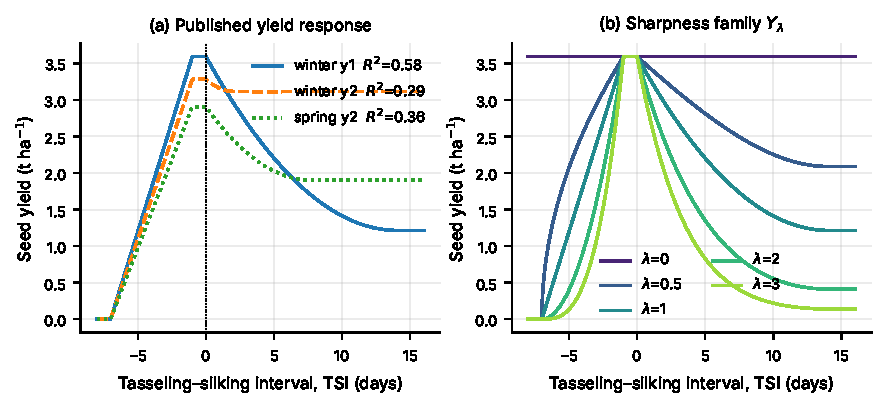
\includegraphics[width=\columnwidth]{../figs/fig1_yield_curve.pdf}
\caption{(a) Published yield--TSI regressions~\cite{marahatta2025}, with the
negative-TSI side supplied by the floral-overlap term. (b) The sharpness
family of \eqref{eq:sharp}; $\lambda = 1$ is the published response.}
\label{fig:curve}
\end{figure}

\subsection{Decision problem}

Let $x_{i,d,o} \in \{0,1\}$ indicate that field $i$ is sown with female day
$d$ and male offset $o \in \mathcal{O}$, and let $V(d,o)$ be the days on which
the crew must attend. Stage~1 solves
\begin{align}
\max \quad & \sum_{i \in \mathcal{F}} \sum_{d \in \mathcal{T}} \sum_{o \in \mathcal{O}}
  a_i \, \mathbb{E}_{\xi}\!\left[ Y_\lambda(\TSI_i(d,o,\xi)) \right] x_{i,d,o}
  \label{eq:obj}\\
\text{s.t.}\quad
& \sum_{d}\sum_{o} x_{i,d,o} \le 1, \qquad \forall i \in \mathcal{F}
  \label{eq:once}\\
& \sum_{i}\sum_{(d,o)\,:\, t \in V(d,o)} x_{i,d,o} \le K,
  \qquad \forall t \in \mathcal{T}
  \label{eq:cap}\\
& x_{i,d,o} = 0 \quad \text{if } d + o \notin \mathcal{T},
\end{align}
where $\xi$ indexes weather scenarios. Constraint~\eqref{eq:cap} is what
couples the fields: it is the reason a decision about one field changes the
biology of another.

Stage~2 is a policy $\Psi$ mapping the information available on day $t$ to a
revised assignment for the fields not yet sown. Writing $\mathcal{I}_t$ for
that information set, we impose \emph{non-anticipativity}:
\begin{equation}
\Psi(t,\xi) = \Psi(t,\xi') \quad \text{whenever} \quad
\mathcal{I}_t(\xi) = \mathcal{I}_t(\xi').
\label{eq:nonantic}
\end{equation}
Two scenarios that are indistinguishable from what has been observed must
receive the same decision. Without~\eqref{eq:nonantic} a rolling-horizon
policy can quietly consult the future and any measured benefit is
meaningless.

% =========================================================================
\section{Strategies}
% =========================================================================

We compare five policies. All share one execution engine, so differences
cannot come from differing accounting.

\begin{description}
\itemsep1pt
\item[\textbf{S1 Conventional.}] Fields in a fixed order, started as early as
the crew allows, with one rule-of-thumb male offset applied everywhere. This
represents current practice.
\item[\textbf{S2 Static (EV).}] Problem~\eqref{eq:obj}--\eqref{eq:cap} solved
once against a single mean-weather forecast. This is the expected-value
solution.
\item[\textbf{S3 Static (robust).}] Solved once against a weather ensemble
with rain-induced slippage priced in. This is deliberately a \emph{strong}
baseline: it is the best plan obtainable without ever looking at the season
as it unfolds.
\item[\textbf{S4 Dynamic.}] Starts from the S3 plan and re-optimises every
$q$ days on a conditional ensemble formed by historical analogue, described
below, subject to~\eqref{eq:nonantic}.
\item[\textbf{S5 Wait-and-see.}] Solved with perfect foreknowledge of the
realised season. Not implementable; it bounds what any policy could achieve.
\end{description}

Following stochastic programming convention~\cite{birge} we report
$\VSS = \text{S3} - \text{S2}$, the value of modelling uncertainty at all;
$\text{S4} - \text{S3}$, the value of adaptivity, which is the quantity this
paper is about; and $\EVPI = \text{S5} - \text{S4}$, the residual worth of
perfect information.

\subsection{Conditioning without inventing weather}

A rolling-horizon policy needs a conditional forecast: given the season so
far, what are the plausible remainders? The usual device is to splice the
observed prefix onto sampled climatological futures, and it is unavailable
here --- flowering comes from a crop model indexed by year, so a spliced
season is not one the model can run, and a scheduler built on one would be
optimising against phenology that does not exist.

We therefore condition by \emph{historical analogue}. On each replanning day
the season to date is compared with the same calendar stretch of every other
year on record, scored on accumulated thermal time and cumulative rainfall,
and the closest $m$ years become the forecast ensemble. Early in the window
the record is short and almost every year is a plausible analogue; as the
season advances the set narrows, and that narrowing \emph{is} the information
the adaptive policy has and the static plan does not. Non-anticipativity
holds by construction: similarity is computed only over elapsed days, and the
realised season's future is never read. This is, we believe, the natural way
to replan in-season whenever the objective is supplied by a year-indexed
process model, and it is not specific to this crop.

\subsection{Two details that decide the outcome}

Preliminary runs had the dynamic policy performing \emph{worse} than the
static one, for two reasons worth recording because both are easy to get
wrong. First, a rolling horizon free to reassign everything at each step can
defer a field indefinitely, each revision locally attractive, until the
window closes and the field is never sown; we freeze any operation within
$\ell$ days of its scheduled date, which is also operationally realistic.
Second, if the scenario-averaged objective already prices in rain slippage,
the optimiser must not \emph{also} forbid days that might be wet --- doing
both charges the same risk twice. We additionally adopt a revision only when
it improves the expected objective over the plan already in hand.

\begin{algorithm}[t]
\caption{Rolling-horizon execution}
\label{alg:roll}
\small
\begin{algorithmic}[1]
\STATE $P \leftarrow$ Stage-1 plan (S3); $D \leftarrow \emptyset$
\FOR{$t = 1$ \TO $T$}
  \IF{$t \bmod q = 0$ \AND $P \ne \emptyset$}
    \STATE build conditional ensemble from $\mathcal{I}_t$ \COMMENT{obeys \eqref{eq:nonantic}}
    \STATE freeze operations due within $\ell$ days
    \STATE $P' \leftarrow$ re-solve \eqref{eq:obj}--\eqref{eq:cap} over unsown fields
    \STATE \textbf{if} $\mathrm{score}(P') > (1+\epsilon)\,\mathrm{score}(P)$ \textbf{then} $P \leftarrow P'$
  \ENDIF
  \STATE execute operations due by $t$, in planned order, while the field is
         trafficable and crew capacity remains; otherwise defer
\ENDFOR
\STATE \textbf{return} $\sum_i a_i Y_\lambda(\TSI_i)$ from realised sowing days
\end{algorithmic}
\end{algorithm}

% =========================================================================
\section{Experimental Design}
% =========================================================================

\subsection{Site and weather}

We study Ranebennur taluk, Haveri district, Karnataka
($14.60^\circ$N, $75.60^\circ$E, 597~m), which together with the adjacent
Ranebennur--Haveri belt is one of India's principal hybrid maize seed
production areas. Weather is twenty-one complete observed seasons, 2005--2025,
from NASA POWER: daily maximum and minimum temperature, precipitation and
solar radiation on the $0.5^\circ$ grid cell containing the site. Nothing is
generated. Every season a strategy is evaluated on is a season that happened.

Seed crops here are grown in the \emph{rabi} season, sown between
1~October and 30~November so that flowering falls in the dry December--January
window when pollen is not washed off the tassel. The sowing window is
therefore $T = 61$ days (day of year 274--334), and rain during it is the
disturbance the schedule must absorb. A field is untrafficable on any day
with more than 5~mm of rain and for $\rho_i$ days afterwards, where
$\rho_i \in \{1,2,3\}$ is the field's drainage class.

\subsection{Phenology}

Flowering dates come from CERES-Maize as implemented in
DSSAT-CSM~v4.8~\cite{dssat}, not from the degree-day approximation of
Section~III. For every combination of cultivar, season and sowing day in the
window we ran the model and recorded the simulated anthesis date, giving a
lookup table of $8 \times 21 \times 61 = 10{,}248$ entries; all of them reach
anthesis. Simulations are run without water or nitrogen limitation so that
the table isolates the thermal and photoperiodic control of flowering, which
is the mechanism the scheduler reasons about.

The eight cultivars are taken unmodified from DSSAT's distributed maize
genotype file and span 50.2 to 66.3 days to anthesis at this site. Parent
pairs are drawn from this set so that the two lines of a field flower between
1.5 and 14 days apart, which is the range over which staggered sowing is
actually practised; pairs are sampled across that range so that a farm
contains both easy and difficult crosses. Field areas are drawn from 1.5 to
4.0~ha and drainage classes uniformly.

The crop model, not the scheduler, supplies the reason adaptivity could
matter here: for a fixed pair of parents sown on a fixed date, the gap between
their flowering dates varies across the twenty-one seasons with a standard
deviation of 1.5~days on average over the parent pairs of a farm (median 1.4,
range 0.6--2.3). That variation is weather; it is unknown when the plan is
made; and at the measured penalty the first day of asynchrony costs 9.1\% of
seed yield.

\subsection{Protocol}

Evaluation is leave-one-season-out. Each scored season is held out, the
planning ensemble is drawn from the remaining twenty, and no strategy ever
sees the season it is tested on. Because the number of ensemble members
dominates runtime, we sample eight of the twenty remaining seasons for each
scored season, with a fixed seed so that all five strategies face the same
ensemble.

Every strategy is evaluated on the same held-out seasons and the same farms,
so all comparisons are paired. Each configuration is replicated across three
independently generated farms. We report paired $t$-tests on the $S_4 - S_3$
difference, together with mean differences and the number of farms on which
the difference is positive.

Stage-1 and each replan are solved to proven optimality with CBC. Because the
optimiser is exact, any difference between $S_3$ and $S_4$ is attributable to
adaptivity rather than to search noise, which is not the case when both sides
are solved heuristically. As a check on the machinery we reran the dynamic
strategy with its adoption threshold set so high that no revision is ever
accepted; it reproduced $S_3$ exactly, confirming that the measured gain comes
from adopted revisions and not from an implementation difference between the
two arms.

We vary two things. The first is \emph{resource pressure},
\[
  \pi \;=\; \frac{N \cdot V}{T \cdot K},
\]
the ratio of crew-visits demanded to crew-visits available, where $V = 3$
visits per field under split-male sowing. At $\pi < 1$ the crew has slack; at
$\pi > 1$ some fields cannot be served on their preferred days and the
scheduling problem binds. The second is penalty sharpness $\lambda$, swept at
fixed resource pressure.

% ---------------------------------------------------------------------------
\section{External Validation}
\label{sec:validation}

A simulation is only as good as the biology inside it, so we test the model
against a dataset that played no part in building it.
Chassaigne-Ricciulli \textit{et al.}~\cite{chassaigne2021} report, for six
three-way-cross tropical maize hybrids at CIMMYT's station in Agua Fr\'ia,
Mexico, the parents' accumulated degree days at flowering, the differential
sowing interval they recommend, and a ranking of the six by difficulty of
seed production. None of it entered our model: the yield response comes from
Nepal~\cite{marahatta2025} and the phenology from DSSAT~\cite{dssat}.

Three of our parameters are corroborated. Both studies compute thermal time
identically, above a $10^\circ$C base and truncated at $30^\circ$C. CIMMYT
estimate ``7 days for the total pollen shedding duration,'' the value our
floral-overlap term assumes, and report stigmas receptive about five days
after the onset of female flowering, inside our six-day window --- so the one
component we extended beyond the fitted data is supported by measurements
from another continent. The model's core claim, that the offset needed to
synchronise two parents equals their thermal-time difference divided by the
rate of degree-day accumulation, predicts their recommended offsets with a
mean absolute error of 1.5~days and recovers the correct direction in six
cases of six (Fig.~\ref{fig:cimmyt}(a)); ranking the same hybrids by the
offset our model requires reproduces their own difficulty ordering at
Spearman $\rho = 0.71$ (Fig.~\ref{fig:cimmyt}(b)), suggestive rather than
significant at $n = 6$.

This establishes that the biology driving the scheduler behaves like the
published biology. It does not validate the scheduler: no one has executed
one of our schedules on real fields and weighed the resulting seed. What it
buys is the right to read differences between strategies as differences in
scheduling quality rather than artefacts of a misspecified crop response.

\begin{figure}[t]
\centering
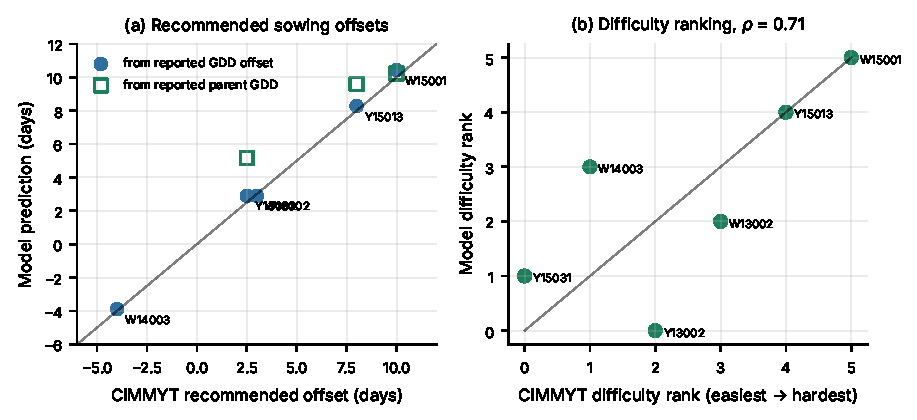
\includegraphics[width=\columnwidth]{../figs/fig7_cimmyt.pdf}
\caption{External validation against CIMMYT's published seed-production
recommendations~\cite{chassaigne2021}. (a) Predicted against recommended
sowing offsets for six three-way-cross hybrids; the line is parity.
(b) Hybrid difficulty ranking.}
\label{fig:cimmyt}
\end{figure}

The same paper also states the assumption this study removes. Recommending
that males be sown on two consecutive dates, it notes that ``it is assumed
that machinery is available to do the sowing, or, in the case of rains after
the first sowing, staff are available to planting.'' The agronomic literature
derives the offsets each hybrid needs and supposes the crew will be free to
deliver them; we ask what happens when one crew serves many fields and rain
closes some of them. We also adopt their two-date male sowing, which raises
the work per field from two crew visits to three.


% =========================================================================
\section{Results}
% =========================================================================

RESULTS_SECTION

% =========================================================================
\section{Discussion}
% =========================================================================

DISCUSSION_SECTION

% =========================================================================
\section{Limitations}
\label{sec:limits}
% =========================================================================

\emph{This is a simulation study.} No seed was produced. The results say
when these schedules are worth \emph{testing} in the field, not that a given
gain will be realised on a given farm.

\emph{The parents are public cultivars.} Flowering comes from CERES-Maize
driven by DSSAT's distributed genotype coefficients, which span a realistic
range of maturities but are not the proprietary inbreds of any commercial
hybrid. A producer's own calibration would shift the required offsets without
changing the structure of the result, which depends on how variable the
parent flowering gap is across seasons rather than on its mean. Flowering is
also simulated without water or nitrogen limitation, which isolates the
thermal control of anthesis; under stress asynchrony would be larger and more
weather-dependent, which would if anything raise the value of adaptivity.

\emph{The yield response is from one site and extended on one side.} The
regression is from Chitwan, Nepal, applied at a Karnataka site; it is the
only published quantitative seed-yield-versus-TSI response we could find, and
Section~\ref{sec:validation} tests its parameters elsewhere rather than
assuming they transfer. The negative-TSI branch is built from reported
floral-window durations, not fitted.

\emph{We model one control lever, and score mass rather than saleable seed.}
Producers correct a flowering gap by staggering sowing \emph{and} by applying
supplementary nitrogen to the late parent~\cite{priyanka2017,patil2026,%
asefa2024}; we model only the first. Modelling the second would also require
replacing our objective, since nitrogen changes seed weight and hence the
size grading and germination on which hybrid seed is actually
sold~\cite{marahatta2025}. A schedule maximising tonnage need not maximise
certifiable seed.

\emph{The scheduler observes weather, not plants, and observation is free.}
Our replanner conditions on thermal time and rainfall to date, whereas a
leaf-number criterion proved more consistent across planting dates in hybrid
rice~\cite{varma2018}. CERES-Maize does represent leaf appearance explicitly
through a phyllochron parameter, so the state we advance is closer to that
criterion than to a hand-computed degree-day rule, but we never feed observed
leaf stage back. Relatedly, each replanning step uses the season to date at
no cost, while learning a field's true state means visiting it and consuming
the capacity the schedule is competing for --- which makes our estimate in
the band where adaptivity already returns nothing optimistic rather than
pessimistic. Crew capacity is likewise a swept parameter, not a measurement,
and rain is the only disruption modelled.

% =========================================================================
\section{Conclusion}
% =========================================================================

CONCLUSION_SECTION

\section*{Reproducibility}
The simulator, the DSSAT driver and anthesis table, the NASA POWER weather
record, the experiment scripts and every result table accompany this
submission and will be released publicly on acceptance. Every biological
parameter is traceable to an open-access publication cited here, and the
validation data of Section~\ref{sec:validation} are quoted verbatim in the
released code so the comparison can be re-checked at source.

\balance
\begin{thebibliography}{99}
\footnotesize

\bibitem{marahatta2025}
S.~Marahatta, R.~Basnet, S.~Bastola, and P.~R.~Dulal,
``Optimizing male inbred sowing for hybrid maize seed production in winter and
spring,'' \textit{Journal of Agriculture and Food Research}, vol.~24,
art.~102350, 2025.

\bibitem{kelly2023}
T.~D.~Kelly, T.~Foster, and D.~M.~Schultz,
``Assessing the value of adapting irrigation strategies within the season,''
\textit{Agricultural Water Management}, vol.~275, art.~107986, 2023.

\bibitem{becker2026}
C.~J.~Becker \textit{et al.},
``Optimizing irrigation and fertilization strategies for crop growth: a
comparative study of genetic algorithm and model predictive control under
weather uncertainty,'' \textit{Archives of Computational Methods in
Engineering}, 2026.

\bibitem{laurent2025}
A.~Laurent \textit{et al.},
``Predicting inbred parent synchrony at flowering for maize hybrid seed
production by integrating crop growth model with whole genome prediction,''
\textit{Crop Science}, 2025.

\bibitem{chassaigne2021}
A.~A.~Chassaigne-Ricciulli \textit{et al.},
``Effective seed yield and flowering synchrony of parents of CIMMYT
three-way-cross tropical maize hybrids,'' \textit{Agriculture}, vol.~11,
no.~2, art.~161, 2021.

\bibitem{fonseca2004}
A.~E.~Fonseca \textit{et al.},
``Simulating potential kernel production in maize hybrid seed fields,''
\textit{Crop Science}, vol.~44, pp.~1696--1709, 2004.

\bibitem{schneider2005}
E.~Schneider,
``Improving the accuracy of kernel set simulation in hybrid maize,''
Ph.D. dissertation, Iowa State University, 2005.

\bibitem{khalilzadeh2022}
Z.~Khalilzadeh and L.~Wang,
``Corn planting and harvest scheduling under storage capacity and growing
degree units uncertainty,'' \textit{Scientific Reports}, vol.~12, no.~1,
pp.~1--20, 2022.

\bibitem{rollinghorizon2023}
F.~Montenegro-Dos Santos \textit{et al.},
``A rolling horizon scheme for rescheduling in agricultural harvest,''
\textit{Computers and Electronics in Agriculture}, 2023.

\bibitem{shared2022}
Y.~Wang \textit{et al.},
``A two-step framework for dispatching shared agricultural machinery with
time windows,'' \textit{Computers and Electronics in Agriculture}, vol.~192,
art.~106607, 2021.

\bibitem{chassaigne2020}
A.~A.~Chassaigne-Ricciulli \textit{et al.},
``Development of seed production technology of CIMMYT tropical single cross
maize hybrids,'' \textit{Agriculture}, vol.~10, no.~8, art.~318, 2020.

\bibitem{asefa2024}
G.~Asefa \textit{et al.},
``Evaluating released maize hybrids parents for yield producibility and
nicking time in mid altitude of western and north western Ethiopia,''
\textit{SVU-Int.\ J.\ Agric.\ Sci.}, vol.~6, no.~3, pp.~1--12, 2024.

\bibitem{priyanka2017}
M.~Priyanka \textit{et al.},
``Influence of synchronization techniques and dates of sowing on nicking in
parental lines of pearl millet hybrid BPMH-3 seed production,''
\textit{Adv.\ Crop Sci.\ Technol.}, vol.~5, no.~4, 2017.

\bibitem{patil2026}
N.~B.~Patil \textit{et al.},
``Optimizing hybrid seed yield in sunflower hybrid KBSH-78 through flowering
synchronization and nitrogen management,'' \textit{J.\ Adv.\ Biol.\
Biotechnol.}, 2026.

\bibitem{varma2018}
R.~L.~Varma \textit{et al.},
``Method optimization for parental line synchronization in hybrid rice seed
production,'' \textit{Int.\ J.\ Curr.\ Microbiol.\ Appl.\ Sci.}, vol.~7,
pp.~1--8, 2018.

\bibitem{sun2023}
J.~G.~Sun \textit{et al.},
``Optimization model and application for agricultural machinery systems based
on timeliness losses of multiple operations,'' \textit{Agriculture},
vol.~13, no.~7, art.~1317, 2023.

\bibitem{bagheri2025}
P.~Bagheri Tookanlou \textit{et al.},
``Predicting readiness of arable land and scheduling of tillage operations
using finite-horizon Markov decision process and Gaussian state space
models,'' \textit{Operational Research}, vol.~25, 2025.

\bibitem{lambrechts2007}
O.~Lambrechts, E.~Demeulemeester, and W.~Herroelen,
``Proactive and reactive strategies for resource-constrained project
scheduling with uncertain resource availabilities,'' \textit{J.\ Scheduling},
vol.~11, pp.~121--136, 2008.

\bibitem{vandevonder2007}
S.~Van de Vonder, E.~Demeulemeester, and W.~Herroelen,
``A classification of predictive-reactive project scheduling procedures,''
\textit{J.\ Scheduling}, vol.~10, pp.~195--207, 2007.

\bibitem{demeulemeester2009}
E.~L.~Demeulemeester and W.~S.~Herroelen,
\textit{Robust Project Scheduling}. Hanover, MA: Now Publishers, 2009.

\bibitem{dssat}
J.~W.~Jones \textit{et al.},
``The DSSAT cropping system model,'' \textit{European Journal of Agronomy},
vol.~18, pp.~235--265, 2003.

\bibitem{birge}
J.~R.~Birge and F.~Louveaux,
\textit{Introduction to Stochastic Programming}, 2nd ed. Springer, 2011.

\end{thebibliography}

\end{document}
